% !TEX TS-program = XeLaTeX
% use the following command: 
% all document files must be coded in UTF-8
\documentclass{textolivre}
% for anonymous submission
%\documentclass[anonymous]{textolivre}
% to create HTML use 
%\documentclass{textolivre-html}
% HTML compile using make4ht
% $ make4ht -c textolivre-html.cfg -u -x article "fn-in,svg,pic-align"   
%
% See more information on the repository: https://github.com/leolca/textolivre

% Metadata
\begin{filecontents*}[overwrite]{article.xmpdata}
    \Title{What are the factors that influence the use of social networks as a means to serve pedagogy?}
    \Author{Melchor Gómez-García \sep Moussa Boumadan \sep Roberto Soto-Varela \sep Ángeles Gutiérrez-García}
    \Language{en}
    \Keywords{Social networks \sep Teacher education \sep Multimedia instruction \sep Information technology}
    \Journaltitle{Texto Livre}
    \Journalnumber{1983-3652}
    \Volume{14}
    \Issue{1}
    \Firstpage{1}
    \Lastpage{16}
    \Doi{10.35699/1983-3652.2021.25420}

    \setRGBcolorprofile{sRGB_IEC61966-2-1_black_scaled.icc}
            {sRGB_IEC61966-2-1_black_scaled}
            {sRGB IEC61966 v2.1 with black scaling}
            {http://www.color.org}
\end{filecontents*}



\journalname{Texto Livre: Linguagem e Tecnologia}
\thevolume{14}
\thenumber{1}
\theyear{2021}
\receiveddate{\DTMdisplaydate{2020}{09}{23}{-1}} % YYYY MM DD
\accepteddate{\DTMdisplaydate{2020}{12}{3}{-1}}
\publisheddate{\DTMdisplaydate{2020}{12}{22}{-1}}
% Corresponding author
\corrauthor{Melchor Gómez-García}
% DOI
\articledoi{10.35699/1983-3652.2021.25420}
% Abbreviated author list for the running footer
\runningauthor{Gómez-García et al.}
\editorname{Daniervelin Pereira}

\title{What are the factors that influence the use of social networks as a means to serve pedagogy?}
\othertitle{Quais são os fatores que influenciam a utilização das redes sociais como meio para servir a pedagogia?}
% if there is a third language title, add here:
%\othertitle{Artikelvorlage zur Einreichung beim Texto Livre Journal}

\author[1]{Melchor Gómez-García \orcid{0000-0003-3453-218X} \thanks{Email: \url{melchor.gomez@uam.es}}}
\author[1]{Moussa Boumadan \orcid{0000-0003-3334-1007} \thanks{Email: \url{moussa.boumadan@uam.es}}}
\author[2]{Roberto Soto-Varela \orcid{0000-0003-2105-5580} \thanks{Email: \url{rsoto@nebrija.es}}}
\author[1]{Ángeles Gutiérrez-García \orcid{0000-0001-7376-6064} \thanks{Email: \url{nines.gutierrez@uam.es}}}

\affil[1]{Universidad Autónoma de Madrid, Espanha.}
\affil[2]{Nebrija University, Espanha.}

\addbibresource{article.bib}
% use biber instead of bibtex
% $ biber tl-article-template

% set language of the article
\setdefaultlanguage[variant=british]{english}
\setotherlanguage[variant=brazilian]{portuguese}

% for spanish, use:
%\setdefaultlanguage{spanish}
%\gappto\captionsspanish{\renewcommand{\tablename}{Tabla}} % use 'Tabla' instead of 'Cuadro'

% for languages that use special fonts, you must provide the typeface that will be used
% \setotherlanguage{arabic}
% \newfontfamily\arabicfont[Script=Arabic]{Amiri}
% \newfontfamily\arabicfontsf[Script=Arabic]{Amiri}
% \newfontfamily\arabicfonttt[Script=Arabic]{Amiri}
%
% in the article, to add arabic text use: \textlang{arabic}{ ... }


%\newcolumntype{b}{X}
%\newcolumntype{m}{>{\hsize=.6\hsize}X}
%\newcolumntype{s}{>{\hsize=.35\hsize}X}
\newcolumntype{b}{>{\hsize=2.3\hsize}X}
\newcolumntype{m}{>{\hsize=1.1\hsize}X}
\newcolumntype{s}{>{\hsize=.5\hsize}X}

\begin{document}
\maketitle

\begin{polyabstract}
\begin{english}
\begin{abstract}
Social networks are a key element in young people's and teenagers' leisure time. But their influence goes beyond the field of entertainment further reaching educational and training environments. These tools can support and improve student learning, but it is clear that they can also be an inconvenience or a potential danger for the youth. The purpose of this research is to describe the profiles of teachers who use social networks as resources for their teaching, both inside and outside the classroom. It also seeks to know the characteristics that influence their incorporation as learning elements. For this reason, a secondary exploitation of the PISA 2018 database is carried out. It contains the data of 21,621 teachers of the secondary education level from the 19 regions of Spain. Multilevel analysis is used as a method of data analysis. The results point out differences in use according to the Autonomous Communities, showing the importance of the age of the teacher and the number of years of experience, both for their use in the classroom and to cover their training needs. Quality teaching requires a commitment to technological resources; therefore, decisive to know these elements in order to design teachers and educational institutions.

\keywords{Social networks \sep Teacher education \sep Multimedia instruction \sep Information technology.}
\end{abstract}
\end{english}

\begin{portuguese}
\begin{abstract}
As redes sociais são um elemento-chave nos tempos livres dos jovens e dos adolescentes. Mas a sua influência vai para além do campo do entretenimento, atingindo o ambiente educativo e de formação. Essas ferramentas podem apoiar e melhorar a aprendizagem dos estudantes, mas é evidente que também podem ser um incômodo ou um perigo potencial para os jovens. O objetivo desta investigação é descrever os perfis dos professores que utilizam as redes sociais como recursos para o seu ensino, tanto dentro como fora da sala de aula. Procura também conhecer as características que influenciam a sua incorporação como elementos de aprendizagem. Por esta razão, é realizada uma exploração secundária da base de dados PISA 2018. Ela contém os dados de 21.621 professores do ensino secundário das 19 regiões de Espanha. A análise multinível é utilizada como um método de análise de dados. Os resultados apontam para diferenças de utilização de acordo com as Comunidades Autônomas, mostrando a importância da idade do professor e o número de anos de experiência, tanto para a sua utilização na sala de aula como para cobrir as suas necessidades de formação. Um ensino de qualidade requer um compromisso com os recursos tecnológicos; por conseguinte, é decisivo conhecer esses elementos para planear professores e instituições de ensino.

\keywords{Redes sociais \sep Formação de professores \sep Instrução multimédia \sep Tecnologia da informação.}
\end{abstract}
\end{portuguese}

% if there is another abstract, insert it here using the same scheme
\end{polyabstract}


\section{Introduction}\label{sec-intro}
The Annual Study of Social Networks \cite{spain2019} points out that in Spain, 85\% of Internet users between the ages of 16 and 65 use social networks. This represents more than 25.5 million users in the country. To get an overview of the extent of the numbers, we can add that the total Spanish population in this age bracket (16-65 years) is 30.9 million people \cite{instituto2018}. Only 5.4 million do not use these digital socialization environments, which represents 17.5\% of the total citizens in this age bracket. Users generate more content quickly and less content that remains documented over time. Under this paradigm, new proposals for the typology of social networks arise, where this form of sharing is favoured, whose main characteristic is to strengthen the link that makes a person constantly aware of new updates, or to be the one who has a recurrent need to update his or her profile with new content. All this without having yet extended the new approaches to connectivity based on 5G technology, which will allow and facilitate new ways of being connected. This facilitates a level of data transfer and ease of access, which will clearly translate into increased connection time in spaces of socialization. We are facing an area in which the forecasts are clearly linked to an exponential growth in a short time, the video format is clearly located as the reference packaging in these new forms of socializing, and the frequency of use of social networks by the vast majority of society is widely extended.

Taking into account these data sets and the new ways of interacting in digital socialization spaces. These spaces can influence many aspects of the lives of individuals who use these applications. \textcite{coll2013} highlights that the skills and competences we develop between the learning we experience, are the result of the different scenarios in which we take part and develop. Considering this casuistry from the educational point of view, we can identify schools as one of these scenarios. But they are not the only ones or online digital spaces have fostered the emergence of a variety of them, thanks to the progress of Information and Communication Technologies (ICT). What we mean is that many young people spend part of their time following referents or "influencers" who can influence them in some way. Therefore, in this new learning ecology described by the author, the most decisive factor is the ability to acquire new knowledge, searching for and generating those conditions to learn in diverse contexts and situations, rather than possessing a dense body of knowledge. This knowledge is updated at a dizzying rate, in these digital niches that have high numbers of visits from young profiles, profiles that we have been calling Millennials or Generation Z, among other categorizations.

In this context, informal training opportunities have an impact on an individual's process of constructing meaning. \textcite{siemens2005}  considers this type of approach as a general characteristic of the whole learning path. Recognizing informal learning opportunities in formal education, takes strength from the number of educational niches that individuals are exposed from their own mobile devices. The great challenge is to be able to ensure, with sufficient evidence, that these networked environments can generate real learning. The interconnection between users in these scenarios is an absolutely necessary condition in itself. Nevertheless, it is not enough \cite{selwyn2010}. The work of teachers in this new learning ecology is a key element in the need to facilitate that learning takes place.

Drawing on specific environments such as social networks and their use as a means of developing a learning experience, \textcite{timothy2016} stresses that these spaces can foster communication between teachers and learners, breaking down geographical barriers and enabling the sharing of diverse interests. On the one hand, it boosts the level of feedback and interactivity in the development of a training opportunity, making access to knowledge more fluid, leading to substantial time saving. Social networks as a tool at the service of pedagogy, favour the development of technical skills and abilities that are fundamental for the acquisition of a digital competence that is essential in today's and tomorrow's society. 

Moreover, they facilitate the increase of fundamental social skills and the development of creative capacity, critical thinking and collaborative work. They are also venues that make it possible to reduce the distance between students and teachers, establishing a task of monitoring and accompanying teachers that has a higher level of immediacy and fluidity \cite{garcia2012,tejedor2012,timothy2016}. The emergence of web 2.0 technologies \cite{oreilly2005}, and in particular social networks, has substantially modified learning ecologies, leading to a prevailing need for new learning pedagogies \cite{casteneda2013}. Pedagogies that take into account that individuals who participate in these spaces must be aware of the learning to which they are being exposed, and be clear about the skills they will be able to acquire. To delimit the evaluative approach, is necessary to know the proposal through which it will be possible to demonstrate what a student has learned \cite{williams2011}.

\begin{sloppypar}
The importance of didactic planning of technology- mediated learning experiences was discussed. Research results in this field \cite{gusman2017,hughes2015} showed that teachers who decide to incorporate ICTs in the planning of their didactic experiences are scarce, and moreover, most of them do not end up being an innovation that can be considered to have an educational impact. This is in accordance with the findings of \textcite{cortina2019}. They state that even if students sometimes have access to technology, they cannot make pedagogically meaningful use of it.
\end{sloppypar}

In this sense, \textcite{gomezgarcia2020} have identified that the aspects of the online training most valuable to teachers are the contents and activities, rather than the format of the proposal or technologies used. In the last decade, many relevant studies have focused on clarifying the impact of the incorporation of professional digital competence in teacher training \cite{instefjord2017}, discovering and analysing basic criteria for the optimal design of training proposals of digital competence, in educational institutions and in teacher training \cite{engen2015}.
This factor that emphasize the importance of technical and pedagogical proficiency in training environments in which we use technology as a means of learning, including social networks. In line with this issue, this study aims to exploit the PISA 2018 database in order to describe the profiles of teachers who use social networks as resources for their teaching, both inside and outside the classroom, determining the characteristics that influence their incorporation as elements of learning.

\section{Methodology}\label{sec-metodologia}

The main objective of this research is to quantify how the digital tools used by teachers are conditioned by the teacher profile observed from variables such as age, teaching experience, gender or nationality. This was done using the PISA 2018 database for Spain to establish, by means of a secondary use of them, which of them had a statistically significant. The results of which were published in December 2019. The aim of the PISA report is to provide comparable data that will enable countries to improve their education policies and results. It involves an analysis that does not evaluate the student, but rather the system in which he or she is being educated.

The sample analysed covers 19 Spanish Autonomous Communities (Andalusia, Aragon, the Balearic Islands, Catalonia, the Canary Islands, Cantabria, Castile-La Mancha, Castile and Leon, the Community of Madrid, the Foral Community of Navarre, the Community of Valencia, Extremadura, Galicia, the Basque Country, the Principality of Asturias, the Region of Murcia and La Rioja, together with the Autonomous Cities of Ceuta and Melilla) and there were 21,621 secondary school teachers participating, specifically at the 15-year level.

36.5\% of the total sample are boys, and 63.5\% are girls. The ages range from 20 to 70 years, with an average of 45.5, with fashion being 50, coinciding with the social phenomenon known as the baby boom of the 1970s.

In the \Cref{fig01} is showed the age distribution of the teachers that participate in the study.

\begin{figure}[htbp]
 \centering
 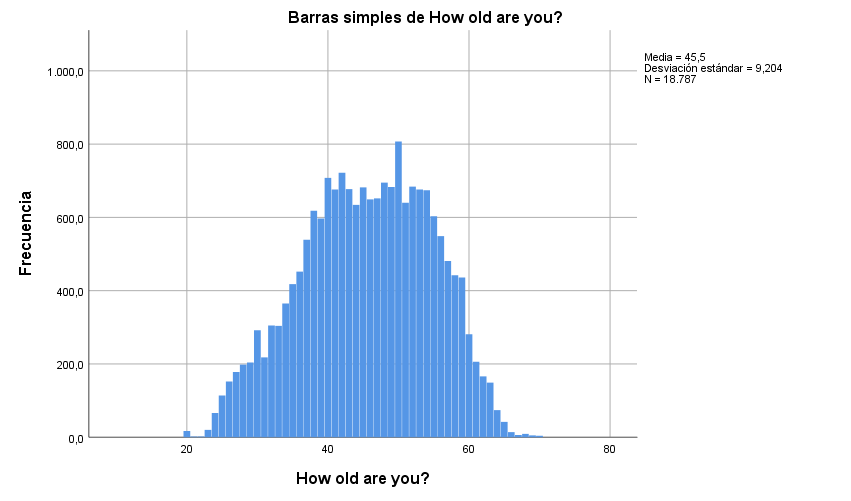
\includegraphics[width=0.75\textwidth]{fig01}
 \caption{Frequency of teacher's age.}
 \label{fig01}
 \source{own elaboration.}
\end{figure}

All participants take a computer-based test. One part of the test is multiple-choice and there is also a part of open-ended questions. It takes about an hour for each participant to answer a questionnaire that focuses on their background, including learning habits, motivation and family.

In our work, we used the macro variable of the PISA study [TC169]: How often did you use the following tools in your teaching this school year? corresponding to the main ‘teacher questionnaire’ (use of information and communication technology at school), and the following country (CNTYD) and identification variables (TC): gender TC001, age TC002, years of teaching experience (TC007).

To develop the methodology, a univariate linear model was calculated on the variable “H\_Social” which is the compilation of the frequencies of use of social networks in education, in the PISA database. It was compared with variables of “teacher's age”, “teacher's sex”, “years of teaching experience” and “teacher's country”, which allowed us to establish the profile of the teacher who uses social media as an educational resource in his/her classes.

The variable TC169Q09HA was recoded for handling, and thus “Never” turned into “0”; “In some lessons” turned into “1”; “In almost every lesson” turned into “2” and “In almost every lesson” turned into “3”.  This approach allowed us to establish an analysis of factorial variances, and contingency tables. 

Finding significance in the explanation of variability in some factors, we focus on those in order to define the profile of the teacher on hypothesis contrasting and mean comparison.

\section{Results}\label{sec-resultados}

\subsection{The age of the teacher and the use of social networks in education}\label{sec-age}

\cref{tbl-tabela-01} shows the different intensities of use of social networks in education, in different age brackets. Each group shows a different average age, so we suspect that there may be a relationship between both variables.

\begin{table}[htpb]
\caption{The age of the teacher and the use of social networks in education.}
\label{tbl-tabela-01}
\begin{tabularx}{\textwidth}{msss}%{XXXX}
\toprule 
Never   & N     & Valid     & 9532 \\
        & Mean  &           & 45.68 \\
        & Std. Deviation &  & 9.131 \\
\midrule
In some lessons & N & Valid & 2955 \\
    & Mean  &   & 44.69 \\
    & Std. Deviation & & 9.069 \\
\midrule
In most lessons & N & Valid & 423 \\
    & & Perdidos & 1 \\
    & Mean  &  & 43.51 \\
    & Std. Deviation & &  9.144\\
\midrule
In every or almost every lesson & N & Valid & 136 \\
    & Mean &    & 43.85 \\
    & Std. Deviation &  & 9.839 \\
\midrule
No Response & N & Valid & 294 \\
    & Mean & & 48.29 \\
    & Std. Deviation & & 8.748 \\
\bottomrule
\end{tabularx}
\source{own elaboration.}
\end{table}

Normal distribution in each of the groups according to the Kolmogorov-Smirnov test, but when analyzing the homoscedasticity, cannot be said for sure that there is an equality of variance between the groups. Therefore, we will apply non-parametric tests, specifically the Kruskall-Wallis test, which confirms the existence of significant age differences between the different groups of social network use.

\Cref{tbl-tabela-02} shows significant elements emerge in the peer-to-peer testing. This allows us to make a difference in two subgroups. A first sub-group formed by teachers who use social networks, and which includes those who use them “In every lesson” and “In most lessons”, and whose mean age is close to 43. And a second sub-group that includes those who “Never” use social networks, which reflects a significant difference in age, and a mean age above 45 years old. The mean age is higher among those teachers with less use of social networks for education.

\begin{table}[htpb]
\caption{Average range of social network usage in education.}
\label{tbl-tabela-02}
\begin{tabularx}{\textwidth}{lXXXXX}
\toprule 
Sample 1-Sample 2 & Contrast test & Error & Control test Dev. & Sig. & Adjusted Sig.\\
\midrule
In most lessons-In every or almost every lesson & 93.524 & 371.070 & -.252 & .801 & 1.000 \\ 
%\midrule
In most lessons-In some lessons &
468.714 & 195.691 & 2.395 & .017 & .100 \\
%\midrule
In most lessons-Never & 894.194 & 187.046 & 4.781 & .000 & .000 \\ 
%\midrule
In every or almost every lesson-In some lessons & 375.190 & 330.135 & 1.136 & .256 & 1.000 \\
%\midrule
In every or almost every lesson-Never &
800.670 & 325.085 & 2.463 & .000 & .000 \\
%\midrule
In some lessons-Never & 425.480 & 79.259 & 5.368 & .000 & .000 \\
\bottomrule
\end{tabularx}

\vspace{1ex}
{\raggedright \footnotesize Asymptotic significances are shown. Significance level is .05. Significance values have been adjusted by Bonferroni correction for several tests. \par}

\source{own elaboration.}
\end{table}
% % essa tabela tem uma nota. Como acrescentar?

\subsection{The use of social networks in the different Autonomous Communities of Spain}\label{sec-use}

\Cref{tbl-tabela-03} shows the different percentages in the use of social network by Autonomous Comunities.

\begin{table}[htpb]
\caption{Social network usage percentage in the different Autonomous Communities.}
\label{tbl-tabela-03}
\centering
\begin{tabular}{ll}
\toprule 
Never & \\ 
\midrule
Andalusia & 68.1 \\ 
Aragon & 74.4 \\
Asturias & 77.3 \\
Balearic Islands & 74.2 \\
Canary Islands & 71.9 \\
Cantabria & 75.0 \\
Castile and Leon & 70.3 \\
Castile-La Mancha & 70.3 \\
Catalonia & 76.2 \\
Extremadura & 68.3 \\
Galicia & 77.0 \\
La Rioja & 65.8 \\
Madrid & 74.2 \\
Murcia & 66.6 \\
Navarre & 76.4 \\
Basque Country & 76.9 \\
Comunidad Valenciana & 74.8 \\
Ceuta & 69.8 \\
Melilla & 65.2 \\
\bottomrule
\end{tabular}
\source{own elaboration.}
\end{table}
%é isto?

\Cref{fig02} shows the process of cluster classification, to explore the social network use by Autonomous Communities and let us make the best decision in terms of the number of subgroups we are going to do.  

\begin{figure}[htbp]
 \centering
 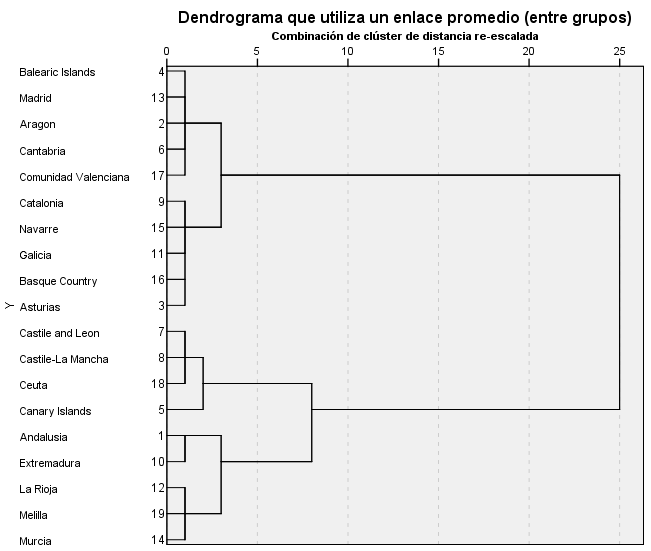
\includegraphics[width=0.75\textwidth]{fig02}
 \caption{Dendogram of social network use by Autonomous Communities.}
 \label{fig02}
 \source{own elaboration.}
\end{figure}

\Cref{tbl-tabela-04} reveals by applying a ranking conglomerate process, we were able to segment the regions into three distinct subgroups with a high degree of accuracy.

\begin{table}[htpb]
\caption{Final Cluster.}
\label{tbl-tabela-04}
\centering
\begin{tabularx}{0.5\linewidth}{XXXX}
\toprule 
& \multicolumn{3}{c}{Clúster} \\ 
& 1 & 2 & 3 \\ 
\midrule
Never Use & 66.80 & 70.58 & 75.64 \\
\bottomrule
\end{tabularx}
\source{own elaboration.}
\end{table}

Social networks are often used with different principles of technology and social communication, and have an integration approach that differs from one classroom to another, depending on the region. Despite the fact that it is not a specific parameter in this work, an initial observation of the graph suggests a relationship between less use of social networks and more rural and unpopulated regions; and more use of social networks in more urban and populated regions. This data is not statistically proven.

\subsection{Gender and use of social networks}\label{sec-gender}

\Cref{fig03} analyze the use of social networks from a gender perspective, we obtain results that seem to indicate that male teachers use social networks more than female teachers in education.

\begin{figure}[htbp]
 \centering
 
\includegraphics[width=0.75\textwidth]{fig03}
 \caption{Gender and use of social networks.}
 \label{fig03}
 \source{own elaboration.}
\end{figure}

\Cref{tbl-tabela-05} reflects, in line with \Cref{fig03}, the use of social networks by gender from absolute values and percentage values.

\begin{table}[htpb]
\caption{Use of social network by gender.}
\label{tbl-tabela-05}
\begin{tabularx}{\linewidth}{XXXXXX}
\toprule 
 & \multicolumn{5}{>{\hsize=\dimexpr5\hsize+5\tabcolsep+\arrayrulewidth\relax}X}{This school year, how often used for teaching: Social media (e.g., Facebook, Twitter)} \\
Are you female or male? & Never & In some lessons & In most lessons & In every or almost every lesson & Total \\
\midrule
Female & 21638 & 10422 & 2450 & 798 & 35308 \\
 & (61.3\%) & (29.5\%) & (6.9\%) & (2.3\%) & (100.0\%) \\
Male & 14857 & 8126 & 2243 & 640 & 25866 \\
 & (57.4\%) & (31.4\%) & (8.7\%) & (2.5\%) & (100.0\%) \\
Total & 36495 & 18548 & 4693 & 1438 & 61174 \\
 & (59.7\%) & (30.3\%) & (7.7\%) & (2.4\%) & (100.0\%) \\
\bottomrule
\end{tabularx}
\source{own elaboration.}
\end{table}
% não sei fazer esta

In \cref{tbl-tabela-06} and \cref{tbl-tabela-07} by means of Chi-square test and Symetric measures, we check if this tendency in the data is statistically consistent, and we get a high significance. These statistician's values indicate a significant relationship between the use of social networks in education and the gender of the teacher.

\begin{table}[htpb]
\caption{Use of social network by gender.}
\label{tbl-tabela-06}
\centering
\begin{tabular}{llll}
\toprule 
& Value & df & Sig \\
\midrule
Pearson Chi-Square & 116.082 & 3 & .000 \\ 
Likelihood Ratio & 115.595 & 3 & .000 \\
Linear-by-Linear Association & 99.049 & 1 & .000 \\
N of Valid Cases & 61174 & & \\
\bottomrule
\end{tabular}
\source{own elaboration.}
\end{table}

\begin{table}[htpb]
\caption{Symmetric Measures.}
\label{tbl-tabela-07}
\centering
\begin{tabular}{lll}
\toprule 
& Value & Aprox. Sig. \\
\midrule
Nominal by Contingency Coefficient & .044 & .000 \\ 
Nominal & & \\
N of Valid Cases & 61174 &  \\
\bottomrule
\end{tabular}
\source{own elaboration.}
\end{table}

\subsection{Experience in teaching}\label{sec-experiencia}
Data on the use of social networks in education according to the number of years of experience of the teacher, are shown below. The first fact we observe is the use of social networks seems to be related to the number of years of teaching experience. In \cref{tbl-tabela-08}, to check if this relationship is situational or statistically significant, we do an Anova test, which gives us the following results.  

\begin{table}[htpb]
\caption{Anova about how many years of work experience do you have? Year(s) working as a teacher in total.}
\label{tbl-tabela-08}
\centering
\begin{tabular}{llllll}
\toprule 
& Sum of Squares & df & Mean Square & F & Sig. \\
\midrule
Between Groups & 7892.648 & 3 & 2630.883 & 26.970 & .000 \\ 
Within Groups & 5884462.679 & 60323 & 97.549 & &\\
Total & 5892355.327 & 60326 & & & \\
\bottomrule
\end{tabular}
\source{own elaboration.}
\end{table}

\Cref{tbl-tabela-09} indicates the group that “uses a lot” and “always uses” do not have different means, but the rest do. The difference in means is significant, and the more social networks are used, the fewer years the teacher has been teaching.

\begin{table}[htpb]
\caption{How many years of work experience do you have? Year(s) working as a teacher in total.}
\label{tbl-tabela-09}
\begin{tabularx}{\textwidth}{mmsssss}
\toprule 
 & & & & & \multicolumn{2}{>{\hsize=\dimexpr2\hsize+2\tabcolsep+\arrayrulewidth\relax}s}{95\% Confidence Interval for Difference}\\\cline{6-7}
 (I) Social media (e.g., Facebook, Twitter) &
 (J) Social media (e.g., Facebook, Twitter) &
 Mean Difference (I-J) &
 Std. Error &
 Sig. &
 Lower Bound &
 Upper Bound \\
\midrule
 Never & In some lessons & $.518^{*}$ & $.090$ & $.000$ & $-.75$ & $-.29$ \\
 & In most lessons & $1.010^{*}$ & $.154$ & $.000$ & $.611$ & $.41$ \\
 & In every or almost every lesson & $1.338^{*}$ & $.268$ & $.000$ & $.652$ & $.03$ \\
In some lessons & Never & $-.518^{*}$ & $.090$ & $.000$ & $-.75$ & $-.29$ \\
 & In most lessons & $.492^{*}$ & $.162$ & $.013$ & $.07$ & $.91$ \\
 & In every or almost every lesson & $.820^{*}$ & $.273$ & $.014$ & $.121$ & $.52$ \\
In most lessons & Never & $-1.010^{*}$ & $.154$ & $.000$ & $-1.41$ & $-.61$ \\
& In some lessons & $-.492^{*}$ & $.162$ & $.013$ & $-.91$ & $-.07$ \\
& In every or almost every lesson & $.328$ & $.300$ & $.693$ & $-.441$ & $.10$ \\
In every or almost every lesson & Never & $-1.338^{*}$ & $.268$ & $.000$ & $-2.03$ & $-.65$ \\
& In some lessons & $-.820^{*}$ & $.273$ & $.014$ & $-1.52$ & $-.12$ \\
& In most lessons & $-.328$ & $.300$ & $.693$ & $-1.10$ & $.44$ \\
\bottomrule
\end{tabularx}

\vspace{1ex}
{\raggedright \footnotesize $^{*}$ The mean difference is significant at the $.05$ level. \par}

\source{own elaboration.}
\end{table}
% não sei fazer essa

In \cref{tbl-tabela-10}, we make the multiple comparisons and form 3 subgroups, which are not as defined as in the case of the age of the teachers.

\begin{table}[htpb]
\caption{How many years of work experience do you have? Year(s) working as a teacher in total.}
\label{tbl-tabela-10}
\begin{tabularx}{\textwidth}{XXXXX}
\toprule 
 & & \multicolumn{3}{>{\hsize=\dimexpr3\hsize+3\tabcolsep+\arrayrulewidth\relax}X}{Subgroups for alpha = $0.05$} \\
Social media (e.g., Facebook, Twitter) & N & 1 & 2 & 3 \\
\midrule
In every or almost every lesson & 1412 & 15.05 & & \\
In most lessons & $4634$ & $15.38$ & $15.38$ & \\
In some lessons & $18323$ & & $15.87$ & $15.87$ \\
Never & $35958$ & & & $16.39$ \\
Sig. & & $.448$ & $.118$ & $.090$ \\
\bottomrule
\end{tabularx}

\vspace{1ex}
{\raggedright \footnotesize The means for the groups are displayed in the homogeneous subsets.\\a. Use the sample size of the harmonic mean = $3974.571$.\\b. Group sizes are not equal. The harmonic mean of the group sizes is used. Type I error levels are notguaranteed. \par}

\source{own elaboration.}
\end{table}
% não sei fazer essa

Looking at the number of years in each of the subgroups, we identified a group that uses social media less as a classroom resource, with an average number of years of experience greater than the other groups. It is highly likely that we find an age-related variable, since the teachers who have more years of teaching experience are usually also the teachers who are older.

\section{Discussion and conclusions}\label{sec-discussao}

The results of this study show three elements of the teacher's profile having an influence on the use of social networks in education.

The first relevant fact is the age of teachers who do not use social networks in teaching, which is significantly different from those who do. If we also look at their mean ages, teachers who use social networks in education are younger than those who do not use them, who are above age 45. This seems to suggest that the older the teacher, the less use is made of this tool in education. This is in line with the research of \textcite{perez2016}, which, although they indicate an absence of difference in digital competence linked to the use of social networks when they look at it from the gender perspective, they do present this difference from the age factor. They conclude that the youngest teachers are those who reach the highest level of digital competence and handling of these tools in pedagogical practice. Nevertheless, \textcite{suarez2013} point out that there is no significant evidence of competence in the area of technology. 

Usually, it is not the age itself that causes a lower level of use of digital resources based on social interactions on the Internet. According to \textcite{correa2015} found that age, gender and educational level influence a better management of the tools that allow social interactions on the network. Demographic variables such as age are influenced by variations over time and context, an issue that requires constant updates \cite{sanchez2010}. In the same vein, \cite{lopez2020} they note that variables such as age, sex and social class affect the assessments made of social networks. The results show that young men are the ones who express positive opinions regarding the use of these media spaces, although they add that these appreciations should be taken in a cautious or careful way. In addition, \textcite{beemt2020} highlight that many studies are not explicit in the demographic description of respondents, leading to the possibility of inferring conclusions that are not very specific, but rather general.

Therefore, it is not age itself that causes the phenomenon, but it is the compendium of multiple variables that are influenced by age \cite{suarez2013,law2008}. We have been able to verify a similar fact when we have analyzed the years of teaching experience, which shows a relationship with the use of social networks similar to that of age. It is clear that these are related factors, but it is difficult to indicate whether the cause is age or the number of years worked. But if we look at the age factor from a general perspective of integration of technologies in learning processes, the older teaching group (between 45 and 55 years) is the one that makes the most varied and frequent use of these tools \cite{area2016}. While \textcite{gomez2012} show that the use of networks for educational purposes usually arises from the initiative of the students, and rarely from the initiative of the teacher.

Gender is the second influential feature. The present study reflects that social networks are a resource that is used more frequently by the male gender, and to a lesser extent by the female gender. This coincides with the findings of \textcite{suarez2013,almerich2011}, which show that both age and gender have a direct impact on the management of social networks in training environments. In turn, these two studies indicate that male teachers have a higher level of competence in the use of ICT, while female teachers are more likely to integrate ICT into their teaching practice.

Nevertheless, when moving from an intermediate to a high level of digital skill in the use of social networks, \textcite{mayor2019} found that gender is the most influential variable. In the present study, the general use of social networks has its highest percentage in the male gender. Contrasting this idea, \textcite{cruz2016} found that women spend more time on social networks, in a general perspective of the use.

The third influential factor is the geographical one. Social networks are integrated to a very different extent in different geographical areas of Spain. Social learning as a methodological approach incorporates many principles of technology and social communication. Although it is not a parameter that is the object of this work, a first observation of the data seems to show a trend towards less use of social networks in both rural and unpopulated regions, and greater use of social networks in urban and populated regions. 

In this regard, \textcite{alcivar2017} showed that there are significant differences between rural areas and those coming from urban areas, pointing out that this is due to the limitations in terms of access to technology and connectivity in rural areas. Even so, if we combine the factor of geographical area and age, \textcite{peral2015} show that socio-demographic variables do not serve to differentiate between elderly people in terms of their use of social networks.

There is no doubt that educational planning cannot ignore the active and social use of social networks \cite{duart2009}. They are one of the main tools for interaction and therefore an excellent opportunity to facilitate communication between educational actors. We must reflect on the enormous educational potential of social networks in education, and the challenge remains to awaken the interest of institutions, teachers and students alike to integrate them as basic teaching tools \cite{casteneda2010}. The study shows significant data regarding the age, sex and years of experience of the teachers. To make this evidence more comprehensible, it would have been interesting to conduct some focus groups with the study participants, which is not an option since this is a secondary use of the database. However, it is a factor to be taken into account for future research.

For all these reasons, it is important to have elements to predict the use of these social spaces from a segmented perspective, and to know which teaching profiles most frequently opt for these tools.

\begin{english}
\printbibliography\label{sec-bib}
\end{english}

\end{document}

